\documentclass[10pt,a4paper]{article}
\usepackage[utf8]{inputenc}
\usepackage[T1]{fontenc}
\usepackage[spanish,es-tabla]{babel}
\usepackage{amsmath}
\usepackage{amsfonts}
\usepackage{amssymb}
\usepackage{makeidx}
\usepackage{graphicx}
\usepackage{lmodern}
\usepackage[left=2cm,right=2cm,top=2cm,bottom=2cm]{geometry}
\author{Ciro Fabian Bermudez Marquez}
\title{Manejo de figuras}
\usepackage{lipsum}


% Libreria de tablas
%\usepackage{caption}				
%\captionsetup{										
%   justification=raggedright
%  ,labelfont={bf}
%}

\begin{document}

\maketitle

\lipsum[1-2]

Como se muestra en la Figura \ref{fig:a2_grafica_seno}, una simple señal senoidal

\begin{figure}[hbtp]
\centering
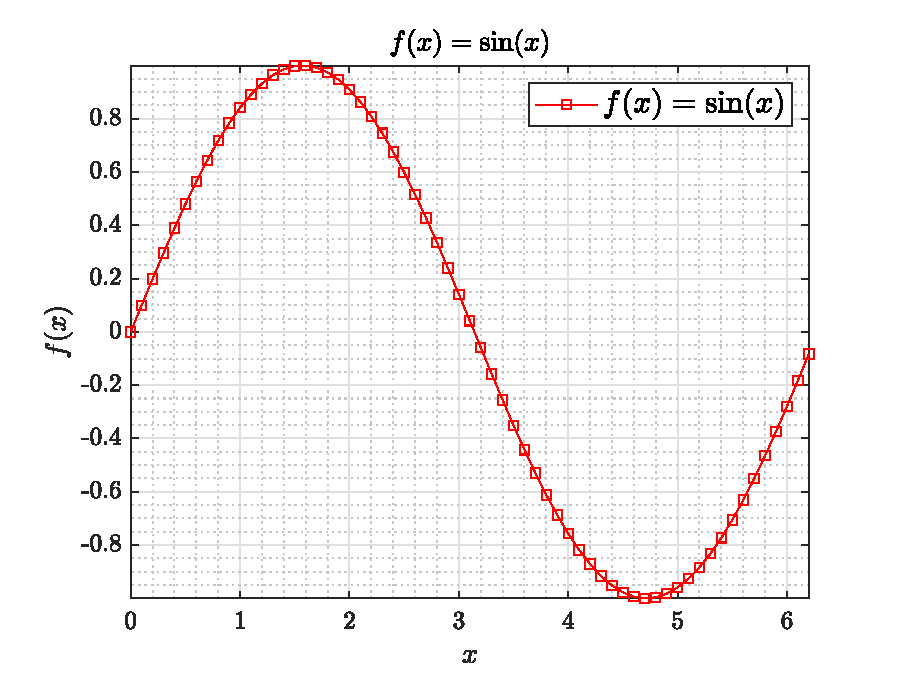
\includegraphics[width=0.5\textwidth]{imagenes/a2_grafica_seno.eps}
\caption{Gráfica de seno.}
\label{fig:a2_grafica_seno}
\end{figure}



Como se muestra en la Figura \ref{fig:a1_meme_fedelobo}, un meme de Fedelobo

	\begin{table}[!hbp]
		\centering
		\begin{tabular}{l  l  l}
			\textbf{Cantidad} &  \textbf{Unidad básica} & \textbf{Símbolo}\\
			\hline
			Longitud 					& metro 		& m		\\
			Masa 						& kilogramo 	& kg	\\
			Tiempo 						& segundo 		& s		\\
			Corriente eléctrica 		& ampere 		& A		\\
			Temperatura termodinámica 	& kelvin 		& K		\\
			Intensidad luminosa 		& candela 		& cd	\\
			\hline
		\end{tabular}
		\caption{Las seis unidades básicas del SI.}
		\label{tab:unidades}
	\end{table}
	


\begin{figure}[hbtp]
\centering
\includegraphics[width=0.5\textwidth]{imagenes/a1_meme_fedelobo.jpg}
\caption{Meme Fedelobo.}
\label{fig:a1_meme_fedelobo}
\end{figure}



% Table generated by Excel2LaTeX from sheet 'Hoja1'
\begin{table}[htbp]
  \centering
    \begin{tabular}{rrrrrrrr}
          & \multicolumn{1}{l}{\textbf{Lunes}} & \multicolumn{1}{l}{\textbf{Martes}} & \multicolumn{1}{l}{\textbf{Miércoles}} & \multicolumn{1}{l}{\textbf{Jueves}} & \multicolumn{1}{l}{\textbf{Viernes}} & \multicolumn{1}{l}{\textbf{Sábado}} & \multicolumn{1}{l}{\textbf{Domingo}} \\
    \hline
    07:00 &       &       &       &       &       &       &  \\
    08:00 &       &       &       &       &       &       &  \\
    09:00 &       &       &       &       &       &       &  \\
    10:00 &       &       &       &       &       &       &  \\
    11:00 &       &       &       &       &       &       &  \\
    12:00 &       &       &       &       &       &       &  \\
    13:00 &       &       &       &       &       &       &  \\
    14:00 &       &       &       &       &       &       &  \\
    15:00 &       &       &       &       &       &       &  \\
    16:00 &       &       &       &       &       &       &  \\
    17:00 &       &       &       &       &       &       &  \\
    18:00 &       &       &       &       &       &       &  \\
    19:00 &       &       &       &       &       &       &  \\
    20:00 &       &       &       &       &       &       &  \\
    21:00 &       &       &       &       &       &       &  \\
    22:00 &       &       &       &       &       &       &  \\
    \end{tabular}%
  \label{tab:addlabel}%
  \caption{Add caption}
\end{table}%




	
\end{document}